\chapter{Event Selection}

\label{ch:selection}

The \acp{LLP} targeted by this search differ in their interactions with the detector from \ac{SM} particles primarily because of their large mass. 
When produced at the energies available at the \ac{LHC}, that large mass results in a low $\beta$ and such slow-moving particles heavily ionize in detector material. 
Each layer of the pixel detector provides a measurement of that ionization, through \ac{ToT}, as discussed in Section~\ref{sec:pixel}. 
The ionization in the pixel detector, quantified in terms of \dedx, provides the major focus for this search technique, both for its discriminating power and also because of the large range of lifetimes where it can be used. The \dedx variable needs to be augmented with a few additional selection requirements to form a complete search. 

Ionization is not currently available in any form during triggering, so this search instead relies on \met to trigger signal events.
Although triggering on \met is not particularly efficient, \met is often large for many production mechanisms of \acp{LLP}, as discussed in Section~\ref{sec:characteristics}.

Ionization is most effective in rejecting backgrounds for well-measured, high-momentum tracks, so some basic requirements on quality and kinematics are placed on the particles considered in this search. 
In particular a newly introduced tracking variable is very effective in removing highly-ionizing backgrounds caused by overlapping tracks. 
A few additional requirements are placed on the tracks considered for \ac{LLP} candidates that increase background rejection by targeting specific types of \ac{SM} particles. 
These techniques provide a significant analysis improvement over previous iterations of ionization-based searches on ATLAS by providing additional background rejection with minimal loss in signal efficiency. 

The ionization measurement with the Pixel detector can be calibrated to provide an estimator of $\beta\gamma$. That estimate, together with the momentum measurement provided by tracking, can be used to reconstruct a mass for each track which traverses the pixel detector. 
That mass variable will be peaked at the \ac{LLP} mass for any signal, and provides an additional tool to search for an excess.
In addition to an explicit requirement on ionization, this search constructs a mass-window for each targeted mass range in order to evaluate any excess of events and to set limits. 
%Construction, calibration, and requirements for the mass variable are discussed in Section~\ref{sec:mass_requirement}.

The strategy discussed here is optimized for lifetimes of $O(1)$ - $O(10)$ ns. 
Pixel ionization is especially useful in this regime as particles only need to propagate through the first seven layers of the inner detector, about 37 cm from the beam axis. 
The search is still competitive with other searches for \acp{LLP} at longer lifetimes, because the primary discriminating variables are still applicable even for particles that do not decay within the detector. 
Although the basic strategy remains the same for all lifetimes, two signal regions are defined to optimize separately for intermediate and long lifetime particles.


% --------------------------------------------------------------------------------

\section{Trigger}

Triggering remains one of the primary difficulties in defining an event selection with high signal efficiency in a search for \acp{LLP}. 
There are no triggers available in the current ATLAS system that can fire directly from a high momentum track with large ionization (Section~\ref{sec:trigger}). 
Although in some configurations a charged \ac{LLP} can fire muon triggers, this requirement introduces significant model dependence on both the allowed lifetimes and the interactions in the calorimeter.

For a search targetting particles which may decay prior to reaching the muon system, the most efficient available trigger is based on missing energy.
As discussed in Section~\ref{sec:characteristics}, signal events can produce \met by two primary mechanisms.
The decays of \rhadrons to neutralinos can produce missing energy when the neutralinos go undetected in the calorimeters.
\acp{LLP} which do not decay before the calorimeters also can produce missing energy because they do not deposit much energy. 
Either case to some extent relies on kinematic degrees of freedom to produce missing energy, as the pair-produced \acp{LLP} tend to balance each other in the transverse plain.
That balance results in a relatively low efficiency for long-lifetime particles, roughly 40\%, and efficiencies between 65\% and 95\% for shorter lifetimes depending on both the mass and the lifetime, as seen in Figure~\ref{fig:trigger_efficiency}. 

\begin{figure}[h]
\centering
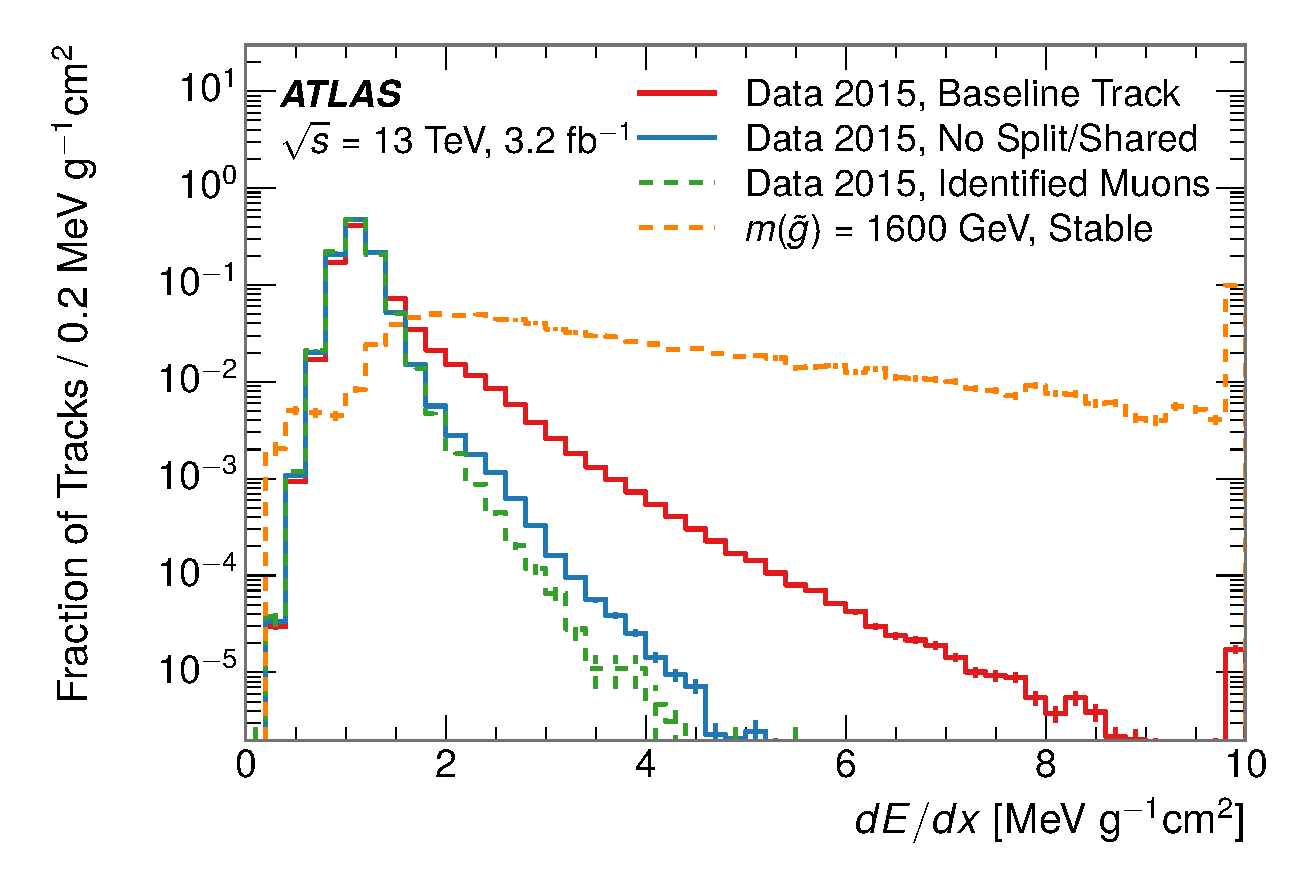
\includegraphics[draft, width=.68\textwidth]{figures/trigger_efficiency.pdf}
\caption{The trigger efficiency of the \met trigger as a function of mass and lifetime.}
\label{fig:trigger_efficiency}
\end{figure}

% ----------------------------------------

\section{Kinematics and Isolation}
\label{sec:track_requirements}

After the trigger requirement, each event is required to have a primary vertex reconstructed from at least two well-measured tracks in the inner detector, each with $\pt > 400$ MeV. 
If more than one such vertex exists, the primary vertex is taken to be the one with the largest summed track momentum for all tracks associated to that vertex. 
The offline reconstructed \met is required to be above 130 GeV to additionally reject \ac{SM} backgrounds.
The transverse missing energy is calculated using fully reconstructed and calibrated offline objects, as described in Section~\ref{sec:missing_energy}. 
In particular the \met definition in this selection uses jets reconstructed with the anti-$k_t$ algorithm with radius $R = 0.4$ from clusters of energy in the calorimeter (Section~\ref{sec:jets}) and with $p_T > 20$ \GeV, as well as reconstructed muons, electrons, and tracks not identified as another object type.

The \met distributions are shown for data and a few simulated signals in Figure~\ref{fig:nm1_met}, after the trigger requirement.
The cut placed at 130 GeV is 95\% efficient for metastable and 90\% efficient for stable particles, because of the missing energy generating mechanisms discussed previously.
The distribution of data in this figure and subsequent figures in this section can be interpreted as the distribution of backgrounds, as any signal contamination would be negligible if present at these early stages of the selection (prior to the final requirement on mass). 
The background falls rapidly with missing energy, motivating the direct requirement on \met for the signal region.
Although a tigher requirement than the specified value of 130 \GeV would seem to increase the search potential from these early distributions, other requirements are more optimal when taken as a whole.
The specific values for each requirement in signal region were optimized considering the increase in discovery reach for tightening the requirement on each discriminating variable. \textbf{NOTE: Is it interesting to discuss the signal region optimization process in detail? I could add another section on how the values were determined, although in truth it is at least partially historical precedence.}

\begin{figure}[h]
\centering
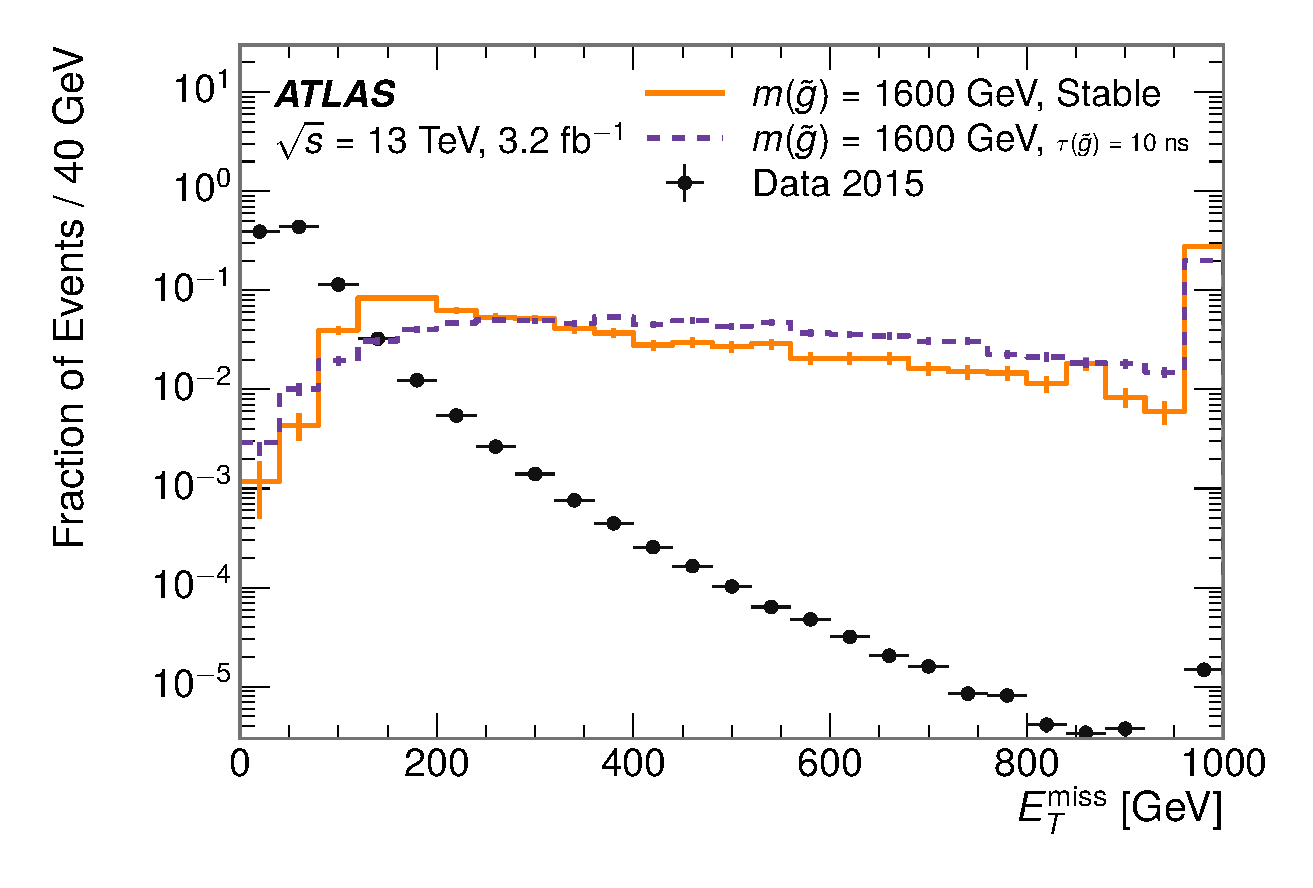
\includegraphics[width=0.68\textwidth]{figures/selection_met_nm1_log.pdf}
\caption{The distribution of \met for data and simulated signal events, after the trigger requirement.}
\label{fig:nm1_met}
\end{figure}

Potential signal events are then required to have at least one candidate \ac{LLP} track.
Although the \acp{LLP} are produced in pairs, many models do not consistently yield two charged particles.
For example, in the \rhadron model highlighted here, only 20\% of events have two charged \rhadrons while 47\% of events have just one.
A signal region requiring two charged candidates could be a powerful improvement in background rejection for a larger dataset, but it is not considered in this version of the analysis as it was found to be unnecessary to reject the majority of backgrounds.

For a track to be selected as a candidate, it must have $p_T > 50$ \GeV and pass basic quality requirements. 
The track must be associated to the primary vertex.
It must also have at least seven clusters in the silicon layers in the inner detector to ensure an accurate measurement of momentum.
Those clusters must include one in the innermost layer if the extrapolated track is expected to pass through that layer.
And to ensure a reliable measurement of ionization, the track is required to have at least two clusters in the pixel detector that provide a measurement of \dedx.

At this point in the selection, there is a significant high-ionization background from multiple tracks that significantly overlap in the inner detector. 
Previous version of this analysis have rejected these overlaps by an explicit overlap rejection between pairs of fully reconstructed tracks, typically by requiring no additional tracks within a cone around the candidate. 
This technique, however, fails to remove the background from tracks that overlap so precisely that the tracks cannot be separately resolved.

A new method, added in Run 2, identifies cluster shapes that are likely formed by multiple tracks based on a neural network classification algorithm. 
The number of clusters that are classified this way in the pixel detector for a given track is called \Nsplit.
As the shape of clusters requires significantly less spatial separation to identify overlaps than it does to reconstruct two fully resolved tracks, this variable is more effective at rejecting backgrounds from overlaps.
Figure~\ref{fig:dedx_nsplit} shows the dependence of ionization on \Nsplit; as \Nsplit increases the mean of \dedx grows significantly up to twice the expected value when $\Nsplit = 4$. 

\begin{figure}[h]
\centering
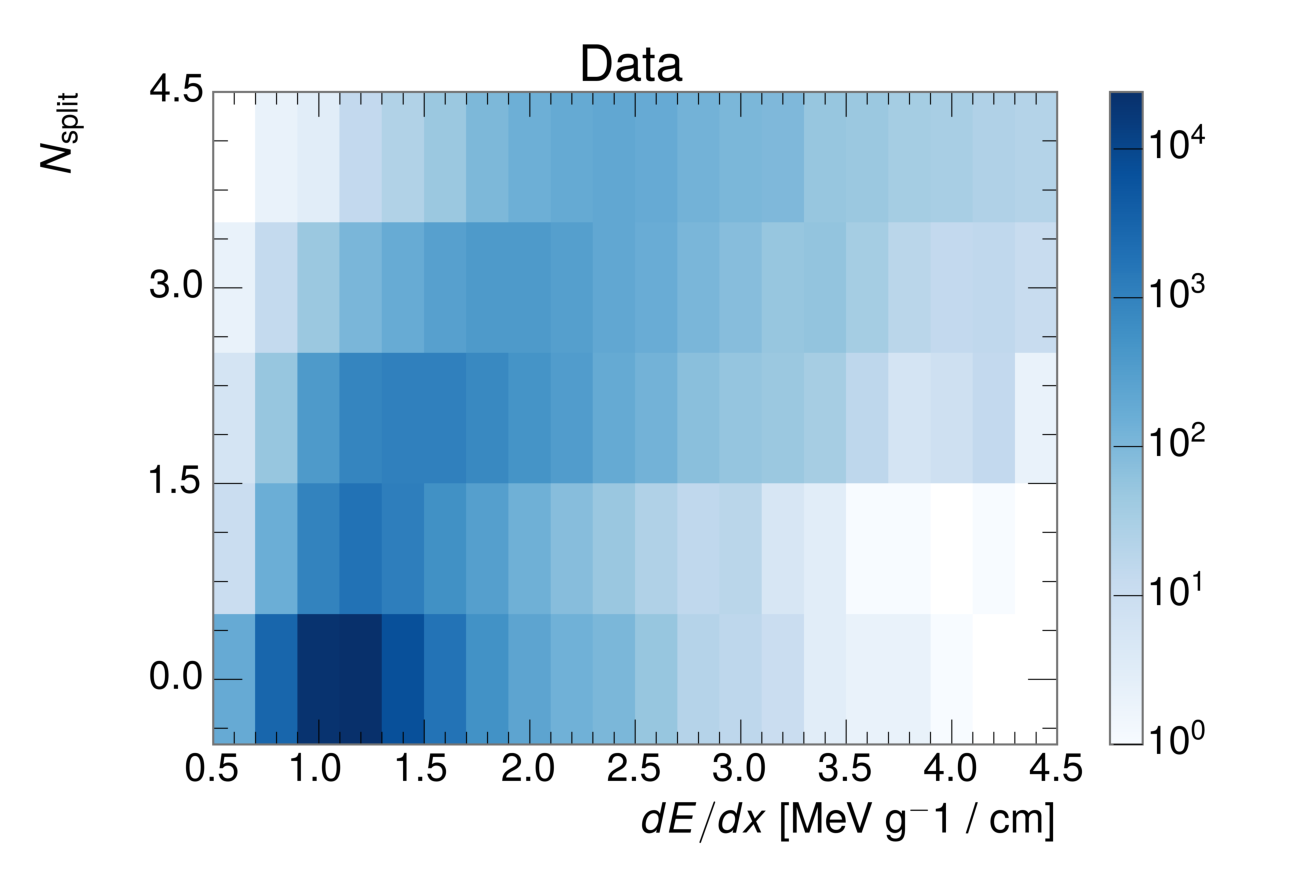
\includegraphics[width=0.68\textwidth]{figures/dedx_nsplit_data.pdf}
\caption{The dependence of \dedx on $N_{\mathrm{split}}$ in data after basic track hit requirements have been applied.}
\label{fig:dedx_nsplit}
\end{figure}

This requirement is very succesful in reducing the long positive tail of the \dedx distributions, as can be seen in Figure~\ref{fig:dedx_isolation}.
Comparing the distribution for ``baseline tracks'', tracks with only the above requirements on clusters applied and before the requirement on \Nsplit, to the distribution with $\Nsplit = 0$, it is clear that the fraction of tracks with large \dedx is reduced be several orders of magnitude.
The isolated tracks are very close to the \dedx distribution of identified muons, which are extremely well isolated on average. 
Figure~\ref{fig:dedx_isolation} also includes the distribution of \dedx in an example signal simulation to demonstrate how effective \dedx is as a discriminating variable with this isolation applied. 
The background falls rapidly for $\dedx > 1.8$ \MeVgcm while the majority of the signal, approximately 90\% depending on the mass, falls above that threshold.

\begin{figure}[h]
\centering
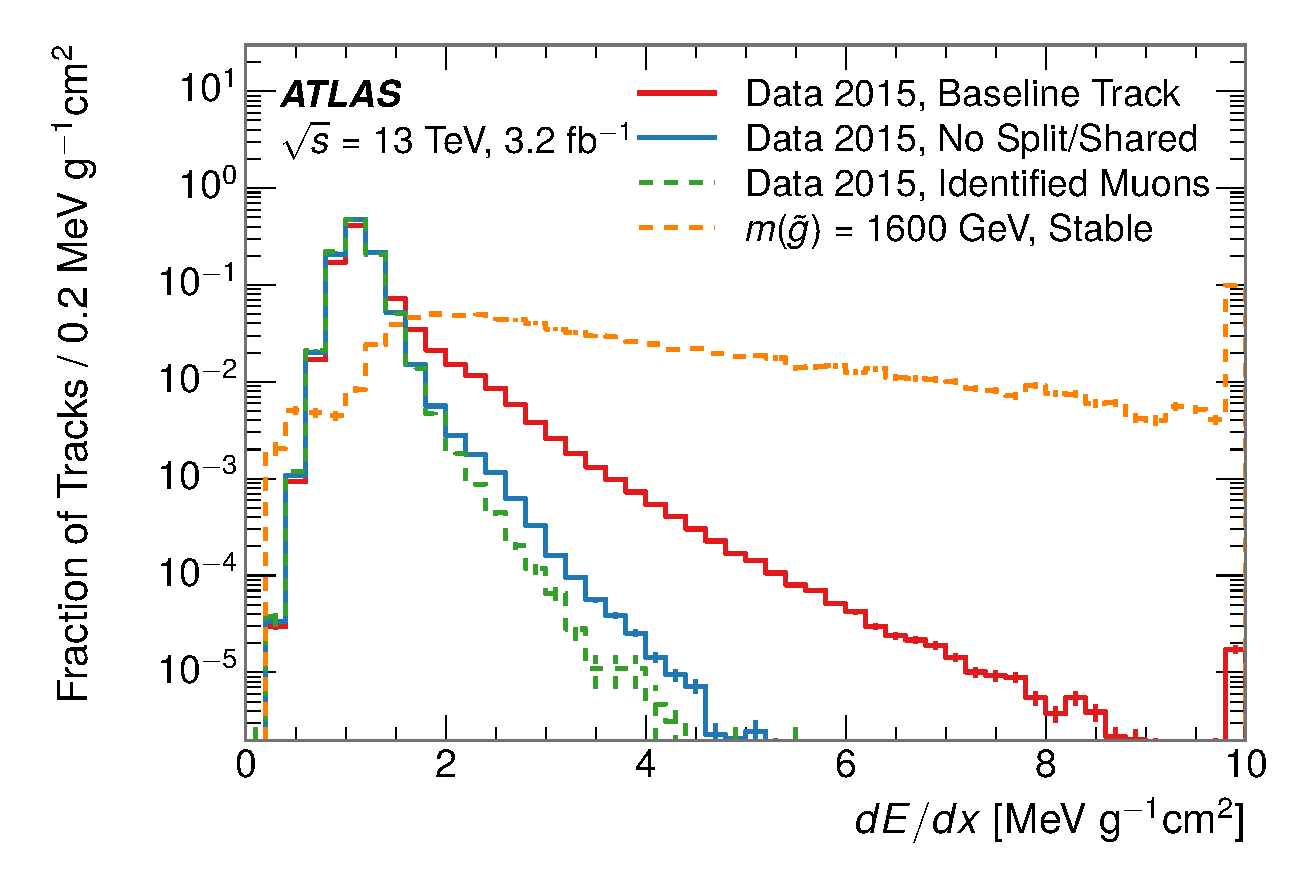
\includegraphics[width=0.68\textwidth]{figures/dedx_isolation.pdf}
\caption{The distribution of \dedx with various selections applied in data and simulated signal events.}
\label{fig:dedx_isolation}
\end{figure}



\begin{figure}[h]
\centering
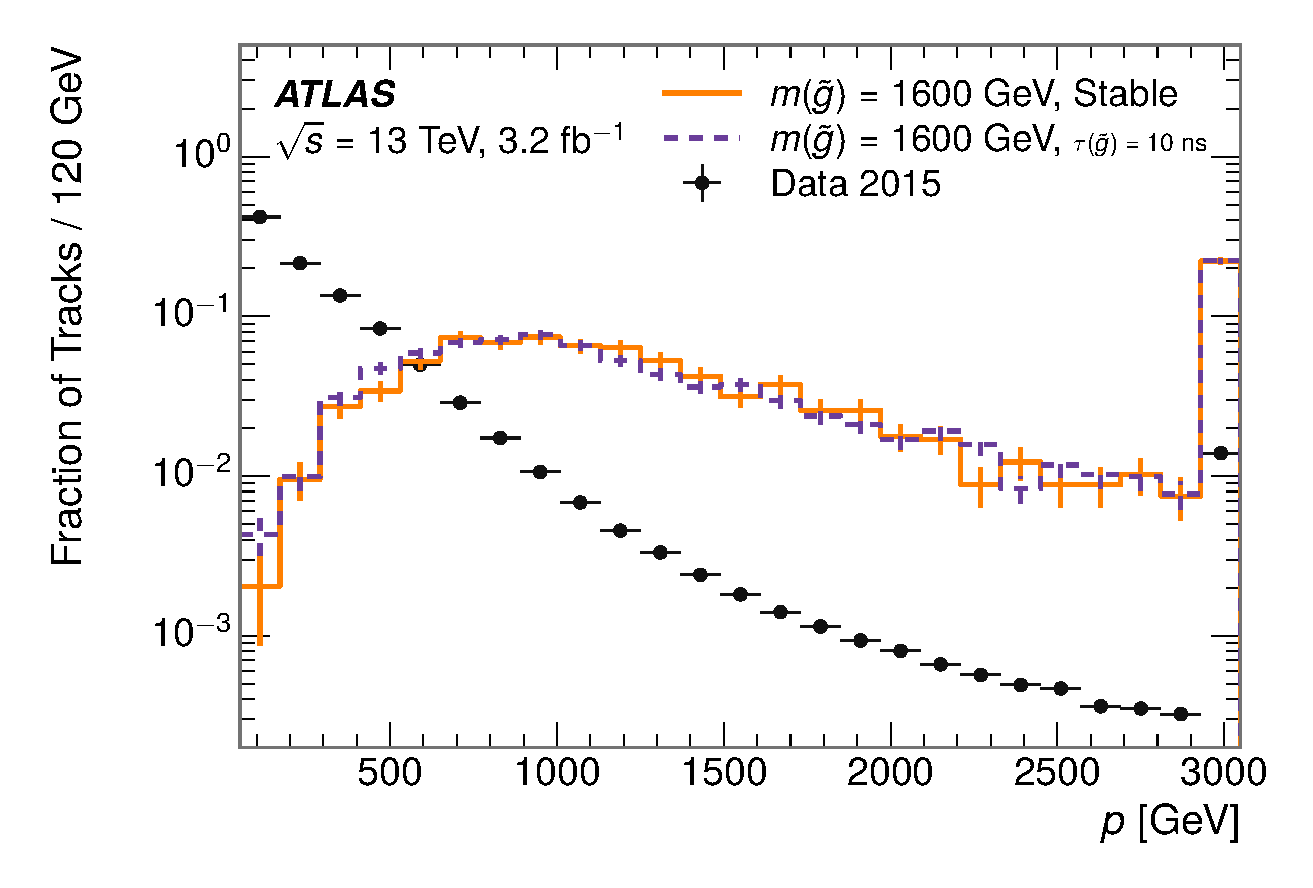
\includegraphics[width=0.68\textwidth]{figures/selection_p_nm1.pdf}
\caption{The distribution of track momentum for data and simulated signal events, after previous selection requirements have been applied.}
\label{fig:nm1_p}
\end{figure}

% ----------------------------------------

\section{Standard Model Rejection}
\label{sec:sm_rejection}



\begin{figure}[h]
\centering
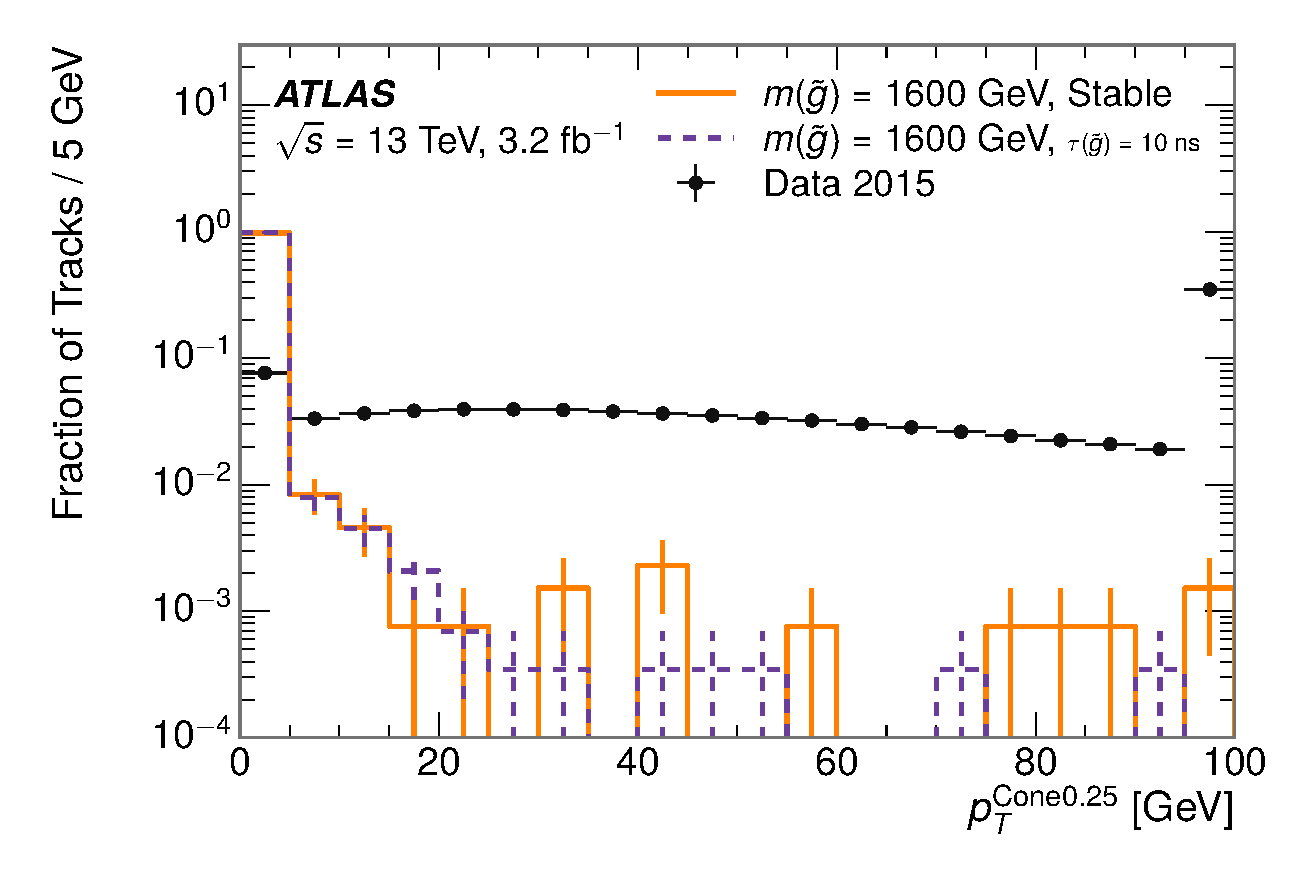
\includegraphics[width=0.68\textwidth]{figures/selection_isopt_nm1.pdf}
\caption{The distribution of summed tracked momentum within a cone of $\Delta R < 0.2$ around the candidate track for data and simulated signal events, after previous selection requirements have been applied.}
\label{fig:nm1_isopt}
\end{figure}

\begin{figure}[htb]
\centering
\subfloat[]{
  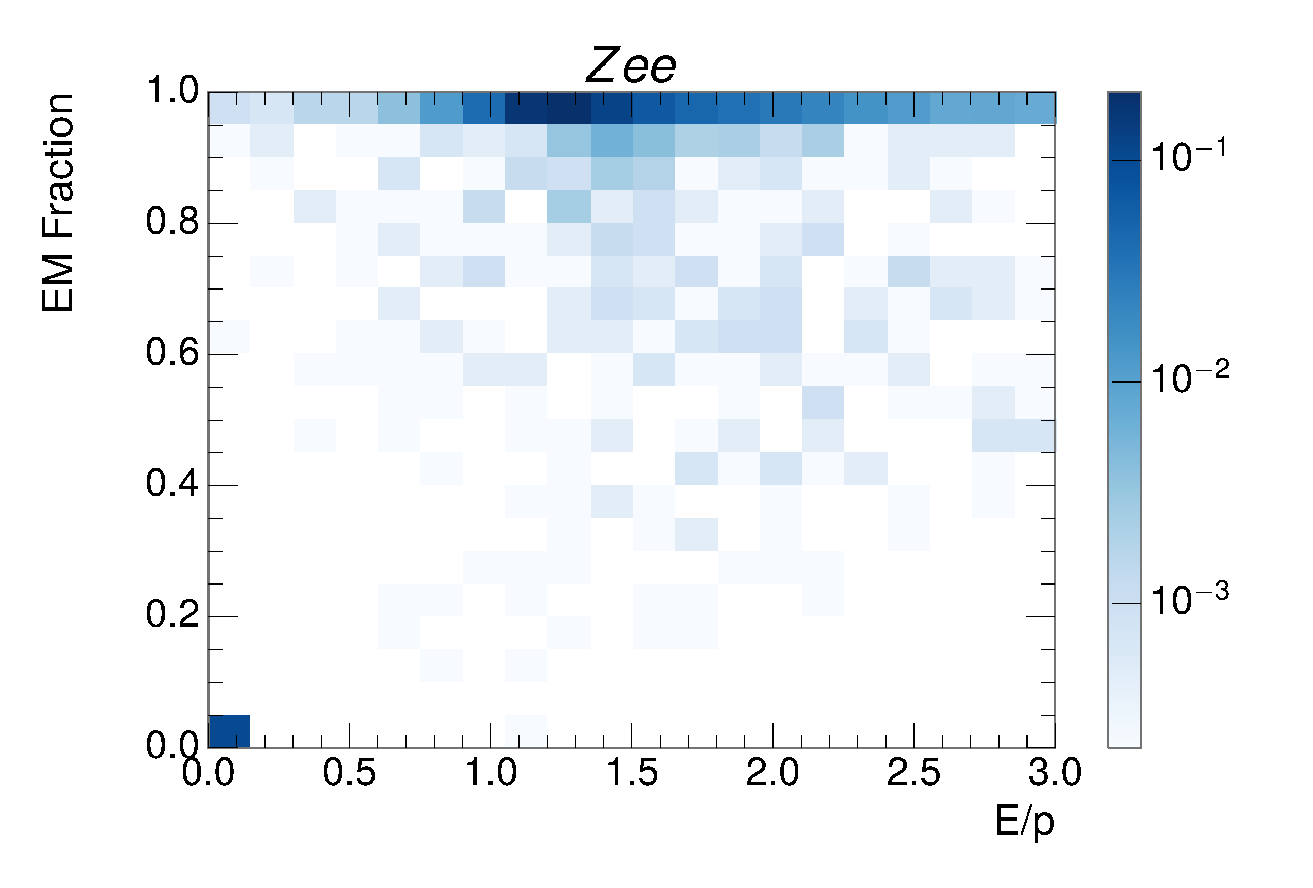
\includegraphics[width=0.48\textwidth]{figures/zee_eoverp_emfrac.pdf}
}
\subfloat[]{
  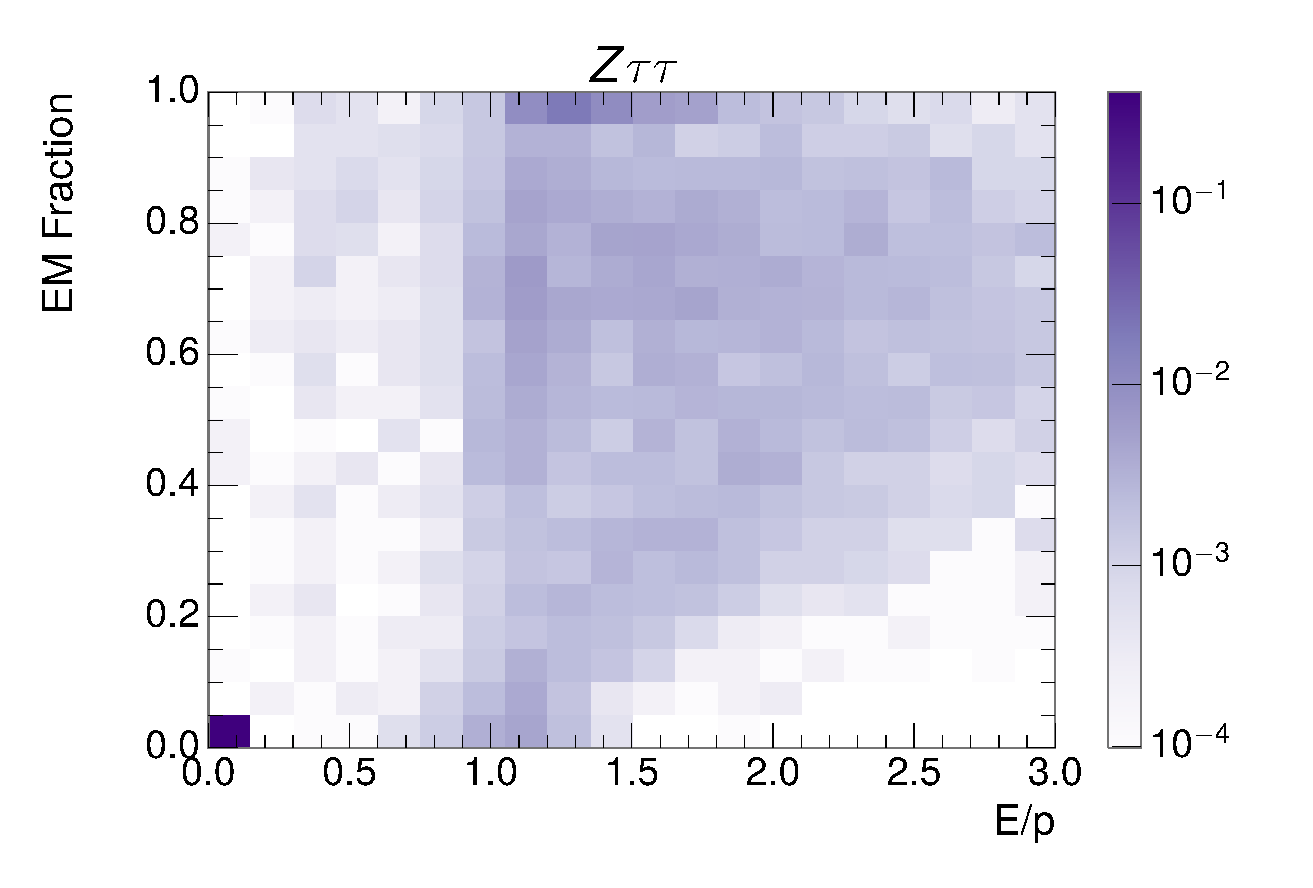
\includegraphics[width=0.48\textwidth]{figures/ztautau_eoverp_emfrac.pdf}
}\\
\subfloat[]{
  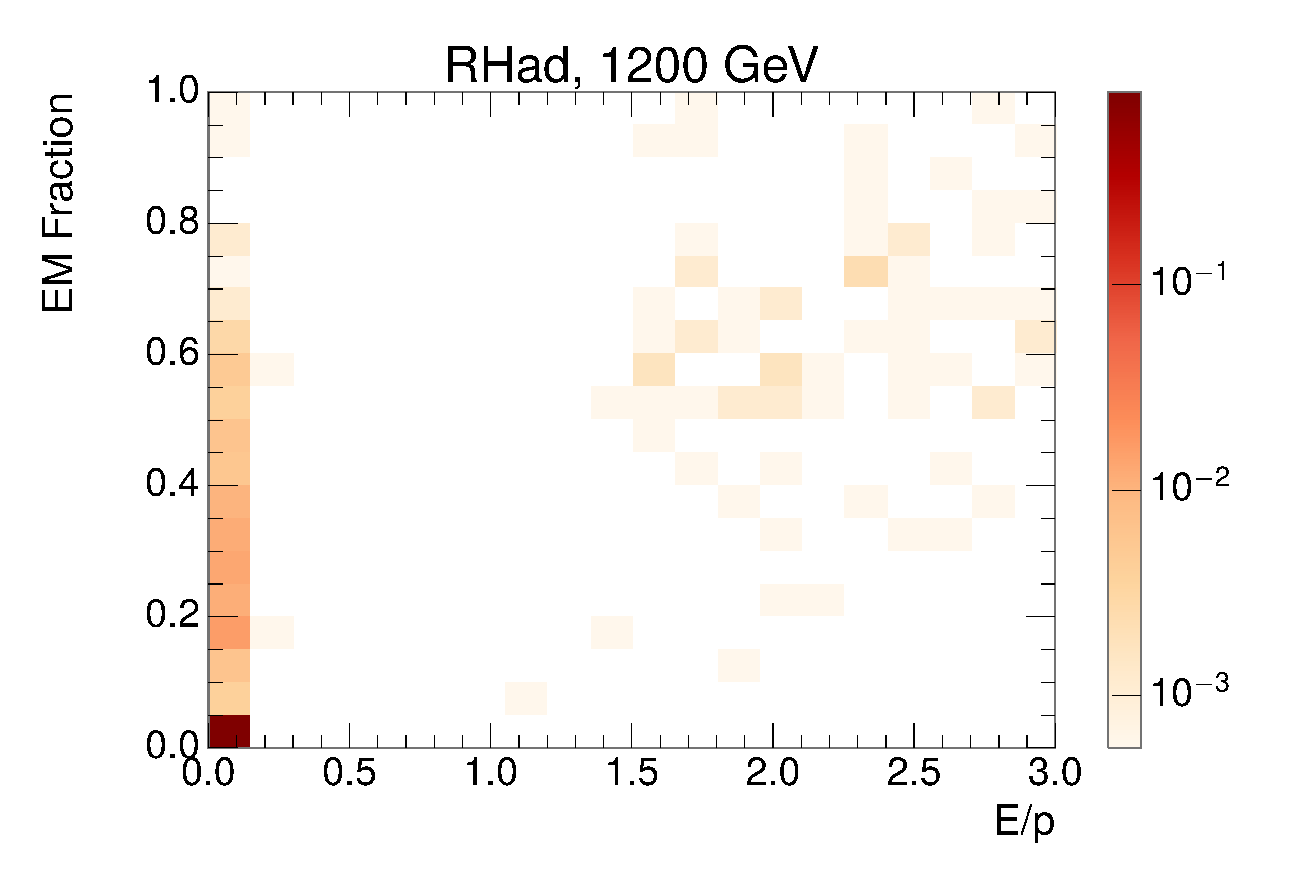
\includegraphics[width=0.48\textwidth]{figures/rhad_eoverp_emfrac.pdf}
}
\caption{The normalized, two-dimensional distribution of $E/p$ and EM fraction for simulated (a) $Z\rightarrow ee$, (b) $Z\rightarrow \tau\tau$ and (c) 1200 GeV R-Hadron events.}
\label{fig:nm1_isopt}
\end{figure}


% ----------------------------------------

\section{Ionization}

\subsection{dE/dx Calibration}

\subsection{Mass Estimation}
\label{sec:mass_requirement}
% ----------------------------------------
